%==========================================================
\chapter{Results}
\label{ch:results}
%==========================================================

This chapter reports the measured results of each component, in the same order as Chapter~\ref{ch:methods}, and closes with the limitations of the evaluation. All numbers come from the project's experiment notebooks, run logs and decision records. Unless stated otherwise, timings were measured on the RTX~5070 machine. Where a result rests on a human judgement rather than on a metric, this is said explicitly.

\section{Data Used in the Evaluation}

Table~\ref{tab:datasets} lists the datasets used to train and evaluate the models. Two features shape the interpretation of the results. First, the operator's own podcast is in Spanish, while most public training data is in English. Second, there is no hand-labelled ground truth for several tasks (relevance, show notes, the ASR reference), so the evaluation combines automatic metrics against a reference model with blind reviews.

\begin{table}[H]
\centering
\caption{Datasets used for training and evaluation.}
\label{tab:datasets}
\small
\begin{tabular}{@{}p{4.2cm}p{5.4cm}p{4.6cm}@{}}
\toprule
\textbf{Dataset} & \textbf{Size} & \textbf{Used for} \\
\midrule
VidChapters-7M subset (en) & 9{,}112 / 900 / 1{,}480 videos (train/val/test) & Chapter boundaries and titles \\
VidChapters-7M subset (es) & 207 videos, split by channel (18 val, 77 test) & Cross-lingual evaluation \\
Operator's episodes & 63 episodes, 40.4\,h, 19{,}348 windows & Relevance pseudo-labels, QA \\
Podcast corpus (M16) & 323 episodes from 20 channels (374\,h selected) & Teacher data for the in-house LLM \\
FineWeb2-HQ / FineWeb-Edu & 5B tokens used (70\% es, 30\% en) & Pretraining of the in-house LLM \\
Market data & 21 channels, 47{,}012 videos, daily snapshots & Market analyses \\
\bottomrule
\end{tabular}
\end{table}

\section{Speech Processing}
\label{s:res-asr}

\subsection*{Transcription}

Table~\ref{tab:whisper} shows the model selection on the new GPU (Section~\ref{s:asr}): WER against the \texttt{large-v3} beam-5 reference on 20 minutes of the operator's audio, the timestamp drift and the time. The setting used on the old GPU (\texttt{large-v3-turbo}, 8-bit, batch 4) was re-measured as the anchor. Batch size barely changes accuracy but changes speed. \texttt{large-v3} in \texttt{int8\_float16} with batch 16 improved the WER by 6.3 points over the anchor, from 17.1\% to 10.8\%, and became the default. It is not the fastest setting: on the 20-minute sample it took 36 seconds against 22 for the anchor, about 1.6 times longer, but it still transcribes a full 43-minute episode at 48 times real time, with a memory peak of 6.5\,GB above the idle level.

The reference was computed in 16-bit floating point, so the advantage of \texttt{int8\_float16} over \texttt{float16} (10.8\% against 14.2\%) cannot come from sharing the reference's numeric format. The bias of the reference towards \texttt{large-v3} variants remains a limitation of this comparison: it favours the chosen model, so the absolute WER values should be read as agreement with the reference rather than as true error rates. No hand-corrected Spanish transcript was available to measure the true error.

\begin{table}[H]
\centering
\caption{Whisper configurations on the RTX 5070 (20 minutes of Spanish podcast audio).}
\label{tab:whisper}
\small
\begin{tabular}{@{}lrrr@{}}
\toprule
\textbf{Configuration} & \textbf{WER} & \textbf{Drift p95} & \textbf{Time} \\
\midrule
turbo, int8, batch 4 (old default, anchor) & 17.08\% & 0.39\,s & 22\,s \\
turbo, int8\_float16, batch 16 & 17.00\% & 0.39\,s & 15\,s \\
turbo, float16, batch 16 & 19.51\% & 0.37\,s & 16\,s \\
large-v3, float16, batch 16 & 14.16\% & 0.31\,s & 34\,s \\
\textbf{large-v3, int8\_float16, batch 16 (chosen)} & \textbf{10.82\%} & 0.34\,s & 36\,s \\
\bottomrule
\end{tabular}
\end{table}

Figure~\ref{fig:whisper} shows the same trade-off graphically. The candidates form two groups: the \texttt{turbo} variants are fast but stay near the anchor's WER, while the \texttt{large-v3} variants are about twice as slow and clearly more accurate. Within each model and precision, larger batches are faster at almost the same WER.

\begin{figure}[H]
\centering
\fig{whisper}
\caption{Accuracy and speed of the Whisper configurations on the RTX 5070. Each series has three points, for batch sizes 4, 8 and 16; batch 16 is always the fastest (leftmost) point.}
\label{fig:whisper}
\end{figure}

On the old GPU, the same protocol had replaced sequential beam search by batched greedy decoding, which halved the transcription time of a 64-minute episode (343 to 165\,s, measured in isolation) with a WER of 13.9\% against 15.1\% for the previous setting. On that machine, then, the faster setting was also slightly more accurate; on the new machine the more accurate setting was chosen at a moderate cost in speed.

\subsection*{Diarization}

On the old GPU, diarization ran at about 18--19 times real time on a 64-minute episode measured in isolation, coexisting with Whisper in 3\,GB thanks to a smaller embedding batch; the CPU ran below real time and was rejected. On the new GPU the batch was raised to 32, which was 22\% faster and produced exactly the same output (a DER of 0.0000 between the two settings). The integration test, on a synthetic conversation between two LibriSpeech speakers, requires at least 90\% of words with the correct speaker. No reference annotation of the operator's episodes exists, so the DER of the deployed pipeline against human labels was not measured.

The review of a full episode found the labels mostly right, with confusion in fast exchanges. An analysis of the stored labels showed that 254 of 3{,}563 Whisper segments (7.1\%, or 9\% of the words) contained more than one speaker. The word labels were correct, but each subtitle cue showed only the majority speaker, so much of the visible confusion was a presentation problem rather than a model error. Splitting cues at speaker changes (Section~\ref{s:asr}) fixed it; the remaining errors are boundary blur in very fast turns. The model found four speakers in an episode with two hosts, and the review confirmed that they were real (guests and audio clips).

\section{Chapter Generation}

\subsection*{Boundaries}

The four BiLSTM configurations reached a validation F1 at 5 seconds between 16.24 and 16.86, so the class weight and the size of the model mattered little (Figure~\ref{fig:chapters-learning}). All of them crossed the baseline after two or three epochs. The best one (projection 384, hidden size 256) beat the TextTiling baseline (16.86 against 7.77), so the trained model was deployed. Table~\ref{tab:chapters} shows the test results, evaluated once.

\begin{figure}[H]
\centering
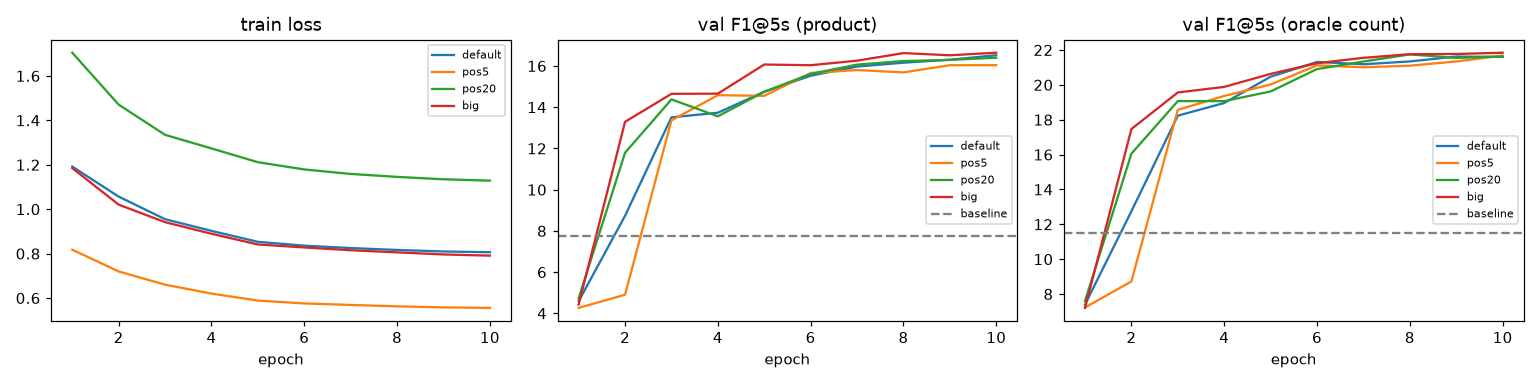
\includegraphics[width=\textwidth]{figures/img/chapters-learning.png}
\caption{Training of the four boundary-model configurations: training loss (left) and validation F1 at 5 seconds in the product and oracle settings (centre, right). The dashed line is the TextTiling baseline. The losses differ in level because the configurations use different positive-class weights.}
\label{fig:chapters-learning}
\end{figure}

\begin{table}[H]
\centering
\caption{Chapter boundaries on the test sets: TextTiling baseline vs.\ trained BiLSTM. F1 in \%; $P_k$: lower is better.}
\label{tab:chapters}
\small
\begin{tabular}{@{}llrrrrr@{}}
\toprule
\textbf{Test set} & \textbf{Method} & \textbf{F1@3s} & \textbf{F1@5s} & \textbf{F1@30s} & \textbf{tIoU-F1} & \textbf{$P_k$} \\
\midrule
\multicolumn{7}{@{}l}{\textit{Product setting (about six chapters per hour)}} \\
English (1{,}480) & Baseline & 6.52 & 8.54 & 21.29 & 12.74 & 0.423 \\
 & BiLSTM & \textbf{14.14} & \textbf{17.89} & \textbf{32.79} & \textbf{18.49} & \textbf{0.366} \\
Spanish (77) & Baseline & 1.87 & 4.32 & 18.92 & 11.90 & 0.417 \\
 & BiLSTM & \textbf{4.99} & \textbf{6.58} & \textbf{23.02} & \textbf{14.84} & \textbf{0.366} \\
\midrule
\multicolumn{7}{@{}l}{\textit{Oracle setting (number of chapters known)}} \\
English & Baseline & 9.66 & 12.89 & 34.91 & 21.96 & 0.413 \\
 & BiLSTM & \textbf{18.22} & \textbf{23.23} & \textbf{46.13} & \textbf{31.57} & \textbf{0.333} \\
Spanish & Baseline & 5.21 & 8.74 & 35.97 & 20.82 & 0.405 \\
 & BiLSTM & \textbf{7.51} & \textbf{11.19} & \textbf{39.88} & \textbf{24.47} & \textbf{0.342} \\
\bottomrule
\end{tabular}
\end{table}

In English the trained model doubles the baseline at the precise tolerances (2.2 times at 3 seconds and 2.1 times at 5 seconds), improves the F1 at 30 seconds and the tIoU-F1 by about 1.5 times, and lowers $P_k$ from 0.423 to 0.366. It also does not degrade on long videos, while the baseline does (Figure~\ref{fig:chapters-duration}). In Spanish it wins on every metric of the table, which shows that the multilingual encoder transfers what the model learnt in English, but the absolute values are low and the per-duration results are erratic: with 12 to 44 videos per bucket, a few videos move the averages by several points. No confidence intervals were computed for these differences, so the Spanish improvement should be read as a consistent direction rather than as a measured margin.

\begin{figure}[H]
\centering
\resizebox{\textwidth}{!}{\fig{chapters-duration}}
\caption{F1 at 5 seconds by video duration on the test sets (product setting). In English the BiLSTM keeps its accuracy on long videos while the baseline degrades; the small Spanish buckets are noisy.}
\label{fig:chapters-duration}
\end{figure}

Two reasons for the weak Spanish results are visible in the data. The Spanish VidChapters transcripts have far fewer sentence breaks, so their units are longer and coarser (Figure~\ref{fig:chapters-examples}, bottom), which makes a 5-second tolerance hard to meet; and there were only 207 Spanish videos. On the 18 Spanish validation videos the baseline had been slightly better at precise placement, a result that the larger test set did not confirm. The numbers must also be read against the ceiling of the unit (83.3 F1 at 5 seconds) and against the fact that the product produces far fewer chapters than creators annotate, which caps recall. Retraining the same recipe on the new GPU reproduced the result within $\pm 0.3$ points (16.64 F1 at 5 seconds on validation). Published results such as Chapter-Llama's are not directly comparable, because they use visual input and a different evaluation subset (Chapter~\ref{ch:soa}).

\begin{figure}[H]
\centering
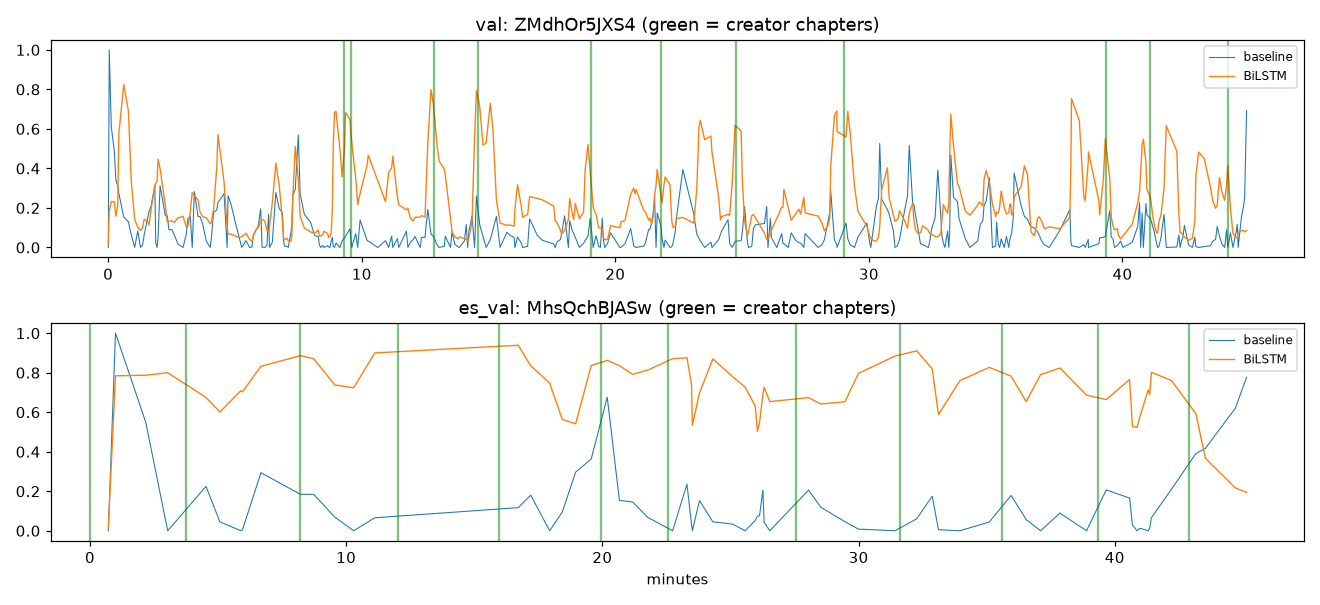
\includegraphics[width=\textwidth]{figures/img/chapters-examples.png}
\caption{Boundary probability per unit for one English (top) and one Spanish (bottom) validation video: TextTiling baseline (blue), BiLSTM (orange) and the creators' chapter starts (green). The BiLSTM produces sharper peaks near the creators' boundaries; the Spanish video has far fewer, longer units.}
\label{fig:chapters-examples}
\end{figure}

\subsection*{Titles}
\label{s:res-titles}

Table~\ref{tab:titles-mt5} shows the fine-tuned mT5 model against the extractive reference (the first eight words of the chapter), on a fixed sample of up to 800 test pairs per language. In English mT5 more than doubles the reference (CIDEr 82.1 against 36.9). In Spanish it barely beats it (49.9 against 44.2), and on a real Spanish episode its titles were not usable: English titles over Spanish speech, repeated words and invented names (Table~\ref{tab:title-examples}).

\begin{table}[H]
\centering
\caption{Chapter titles with mT5-small on the test sets (reference boundaries).}
\label{tab:titles-mt5}
\small
\begin{tabular}{@{}llrrr@{}}
\toprule
\textbf{Test set} & \textbf{Method} & \textbf{BLEU-1} & \textbf{BLEU-4} & \textbf{CIDEr} \\
\midrule
English (800 pairs) & mT5-small & \textbf{18.30} & \textbf{8.83} & \textbf{82.09} \\
 & First 8 words & 8.98 & 3.60 & 36.86 \\
Spanish (620 pairs) & mT5-small & \textbf{9.57} & \textbf{5.46} & \textbf{49.94} \\
 & First 8 words & 8.18 & 4.42 & 44.17 \\
\bottomrule
\end{tabular}
\end{table}

Table~\ref{tab:titles-llm} shows the comparison of local LLMs on validation. All of them produced 100\% of titles in the right language, with no repetitions and no fallbacks, against 90.6\% language accuracy for mT5 in Spanish. The English CIDEr disagreed with the blind review: on a real Spanish episode the review preferred the titles of Qwen3.5-9B for all six chapters, although it had the lowest English CIDEr of the Qwen models. The Spanish CIDEr, on the other hand, agreed with the review, since the 9B model had the highest Spanish CIDEr of all candidates. LLM titles are longer than mT5's (8.8 against 5.1 words on the Spanish test set for the 4B model), and CIDEr penalises length against the creators' short English titles. On the old machine the 9B model did not fit the memory budget, so the 4B model was deployed; after the hardware upgrade a second blind review preferred the 9B model, which is the current default even though it fails the English CIDEr gate (Section~\ref{s:chapters}).

\begin{table}[H]
\centering
\caption{Local LLMs for chapter titles (validation, 150 English and 117 Spanish chapters; CPU time for a real 6-chapter episode on the old machine). English CIDEr gate: at least $0.8 \times 65.9 = 52.7$.}
\label{tab:titles-llm}
\small
\begin{tabular}{@{}lrrll@{}}
\toprule
\textbf{Model} & \textbf{CIDEr en} & \textbf{CIDEr es} & \textbf{Gates} & \textbf{Episode} \\
\midrule
mT5-small & 65.9 & 50.0 & fails (language es) & --- \\
Qwen3.5-2B & 57.8 & 47.6 & pass & 1.9 min \\
Qwen3.5-4B & 55.9 & 44.5 & pass & 4.6 min \\
Gemma4-E4B \cite{gemma4_ref} & 49.3 & 53.8 & fails (CIDEr en) & 4.7 min \\
Salamandra-7B \cite{gonzalezagirre2025salamandra} & 51.6 & 47.2 & fails (CIDEr en) & 5.1 min \\
Qwen3.5-9B & 46.1 & 54.5 & fails (CIDEr en, memory) & 6.9 min \\
Gemma4-E2B \cite{gemma4_ref} & 47.7 & 27.9 & fails (CIDEr en) & 2.5 min \\
\bottomrule
\end{tabular}
\end{table}

\section{Show Notes}

There is no baseline for show notes: a draft can only be checked for validity and judged by a reader. On the first full episode (64 minutes, Spanish, with the 4B model on the CPU), the pipeline produced a valid draft on its first reduce attempt: five title suggestions, fifteen tags, a description of about 110 words with the chapter list, and a two-sentence summary. It took 978 seconds, twice the estimate; moving the prompt processing to the GPU cut it to 351 seconds, and on the new machine with the 9B model a show-notes job takes 52 to 110 seconds per episode. The review approved the draft and noted two weaknesses: two of the five titles repeated chapter titles, because the reduce prompt receives them, and names are only as good as the transcript. In the blind review after the hardware upgrade (two episodes) the 9B drafts were preferred. Because the grammar guarantees that the output is valid JSON, the checks that can still fail are the content rules (lengths, language, minimum numbers of titles and tags); this distinction matters for the in-house language model below.

\section{Relevance Model}
\label{s:res-relevance}

\subsection*{Bootstrap version}

On the first episode, the review confirmed that the five best moments chosen by v0 were good choices. The analysis of the scores, however, showed a property that shaped the trained model: the heuristic and LLM components were weakly and negatively correlated on that episode (Pearson $-0.18$) and uncorrelated over the 19{,}348 windows of 63 episodes ($-0.009$; per episode, between $-0.24$ and $0.27$). The two signals measure different things: the heuristic rewards structure (keywords, questions, speaker changes), while the LLM judges content.

A second finding was the instability of the LLM's integer scores, measured in several ways during the project (Table~\ref{tab:llm-stability}). Moving the 4B model's prompt processing from the CPU to the GPU changed the scores of the same episode substantially, even on identical batches; averaging two shifted passes made them more stable; and even the 9B model's two shifted passes agree only moderately. Even for the teacher, then, relevance at the level of single windows is a noisy judgement.

\begin{table}[H]
\centering
\caption{Stability of the LLM relevance scores (Spearman correlation between two scorings of the same windows).}
\label{tab:llm-stability}
\small
\begin{tabular}{@{}p{2.2cm}p{9.0cm}r@{}}
\toprule
\textbf{Model} & \textbf{Comparison} & \textbf{Spearman} \\
\midrule
Qwen3.5-4B & One pass, CPU vs.\ GPU prompt processing, whole episode & 0.53 \\
Qwen3.5-4B & One pass, CPU vs.\ GPU, identical batches & 0.74 \\
Qwen3.5-4B & Agreement with the original CPU scores: one pass & 0.66 \\
Qwen3.5-4B & Agreement with the original CPU scores: two shifted passes averaged & 0.72 \\
Qwen3.5-9B & Aligned pass vs.\ shifted pass, 49 episodes & 0.49 \\
\bottomrule
\end{tabular}
\end{table}

\subsection*{Trained version}

Table~\ref{tab:relevance} shows the two training iterations on the eight test episodes.

\begin{table}[H]
\centering
\caption{Trained relevance model on the 8 test episodes, compared with the teacher score $s$ (metrics defined in Section~\ref{s:relevance}). Std: standard deviation of the curve.}
\label{tab:relevance}
\small
\begin{tabular}{@{}p{6.2cm}rrrr@{}}
\toprule
\textbf{Model} & \textbf{Spearman} & \textbf{Top-20\%} & \textbf{Top-5} & \textbf{Std} \\
\midrule
Constant & 0.000 & 0.198 & 0.025 & 0 \\
Heuristic alone & 0.545 & 0.478 & 0.275 & 0.175 \\
BiLSTM, iteration 1 (two heads) & 0.396 & 0.390 & 0.125 & 0.003 \\
\textbf{BiLSTM, iteration 2 (exact heuristic + LLM head)} & \textbf{0.652} & \textbf{0.575} & \textbf{0.375} & 0.086 \\
\bottomrule
\end{tabular}
\end{table}

The first iteration failed the offline gate. Its curve had collapsed almost to the mean (standard deviation 0.003), which would have left the Shorts generator nothing to work with. The error analysis, done on training and validation data only, found an optimisation problem rather than a capacity problem: early stopping with a patience of 10 epochs on a noisy validation metric stopped two of the three seeds within the first ten epochs. With a patience of 40 the collapse disappeared, but the two-head score still stayed below the heuristic alone, because the LLM head reproduces the LLM judgement only partially. Since the heuristic is cheap, the second iteration computes it exactly and uses the BiLSTM only for the LLM part (Equation~\ref{eq:relevance-i2}). It passed the offline gate (0.652 against 0.545), and its three seeds agreed within 0.002.

The direct measure of what the student learnt is the Spearman correlation of its LLM head with the teacher's LLM component on the test episodes: 0.38 in the first iteration and 0.41 in the second. In other words, from the text alone the student recovers a moderate part of a judgement on which the 9B teacher agrees with itself at only 0.49 (Table~\ref{tab:llm-stability}). The second iteration also passed the blind A/B test with three wins and two losses, exactly the required minimum. With five episodes this shows that the student was not clearly worse than its teacher, not that it was better. It became the live version.

The trained model scores a 27-minute episode in 1.0 second, against several minutes of LLM time for the teacher. A replay of the Shorts selection on the eight test episodes produced five clips per episode within the length limits, with non-flat curves (14 to 27 peaks per episode after smoothing); 22 of its 40 clips were within 30 seconds of a clip chosen from the teacher's curve. The rendered clips of three test episodes were reviewed and approved.

\section{Shorts}

On the first episode, the Shorts generator produced five clips of 31 to 53 seconds in 55 seconds of processing (9:16 with captions), and the review approved the framing, the cuts, the captions and the choice of moments. Every shot was framed in \textit{crop} mode, because every shot contained a face. The review found one framing error, a blurred hand in the foreground detected as a face with three times the real face's area, which made the crop swing between the hand and the speaker; weighting faces by the fourth power of their confidence fixed it, and a regression test uses the measured boxes. The season run of the hardening milestone (M9) found a second edge case: a closing fade split a clip into one-frame shots and broke the render, fixed with a minimum shot length of 0.5 seconds. On the new machine a Shorts job takes 28 to 46 seconds per episode.

\section{Market Data and Analyses}

\subsection*{Collection}

Of the 22 proposed channels, 21 were loaded; one could not be identified reliably and was left out. Seven of the proposed channel handles were wrong and were corrected by checking each one with the API before loading. The first backfill read 47{,}012 videos for about 970 quota units, and the first daily pull took 47{,}012 snapshots with 941 units, no errors, in 2 minutes and 15 seconds. A typical day uses about 200 units, 2\% of the quota. A manual comparison of 15 videos with the public RSS figures found views within $\pm$0.3\% and identical titles.

The private flows were validated end to end on a test channel. The Analytics connection completed the OAuth flow, pulled data with no errors and reported a revoked token clearly. The Reporting API job was created and, six days later, had downloaded 33 daily reports with no errors: the history that YouTube generates for a new job, starting about a month before its creation, plus the days since. All 33 files contained only the header row, because the test channel had no thumbnail impressions yet, so the CTR value scale could not be verified. Real CTR and retention labels for the trained models therefore do not exist yet; this is the main data limitation of the project.

\subsection*{Analyses}

On the market data collected during development, the channel clustering chose $k = 2$ with a silhouette coefficient of 0.21, which indicates a weak structure; the interface states this so that the map is not over-read. The Spearman correlation of the age- and channel-adjusted residual with video features was 0.30 for video length, 0.16 for a number in the title and $-0.06$ for a question in the title; the interface shows each with its bootstrap interval. The keyword lift placed specific guests and topics at the top and words such as ``live'' or ``covid'' at the bottom. These are associations in observational data and describe what drew audiences in the past, not words that cause views; the interface says so next to each chart. Computing all analyses takes about 9.5 seconds, and an unchanged data fingerprint skips the computation in 0.03--0.1 seconds.

\section{CTR Predictor and Hook Scorer}

Neither heuristic model can be evaluated against real outcomes yet, for the reasons above. They were checked for behaviour. A dry run of the hook scorer on 25 clips of 5 episodes gave scores between 68.5 and 100. The ``dead air'' sub-score was 1.0 for every clip, because the Shorts generator always cuts at the start of a sentence, so on this channel it does not separate clips; framing and direct address carried the ranking, and opening questions were detected correctly. Direct address mostly counted the hosts talking to each other rather than to the viewer, a known limitation. For the CTR predictor, test frames showed that the channel's thumbnails are mostly single-camera close-ups with one face, so the face-count dimension varies less than expected. Both models were reviewed on real episodes and accepted as transparent first versions.

\section{In-House Language Model}

\subsection*{Recipe}

Figure~\ref{fig:ablations} shows the ablations. The higher learning rate passed the adoption rule ($-0.0164$ bpb at no cost). The Muon optimiser was better still ($-0.0240$ against the baseline, at a 2\% throughput cost), so it also passed the rule as written. It was not adopted because every candidate ran at the baseline's learning rate: Muon was only 0.0076 better than the higher learning rate, within the noise expected from single-seed runs, and the combination of Muon with a higher learning rate was not measured. Keeping AdamW with the higher learning rate was the simpler of two close options, and it is the choice that the stage~A run used. The deeper model lost 11\% of throughput for no gain, and the cosine schedule was clearly worse.

\begin{figure}[H]
\centering
\fig{ablations}
\caption{Ablations of the in-house language model at 1B tokens (single seed each). Baseline: 1.0743 bpb. The dashed line is the adoption threshold; the learning rate of $2\times10^{-3}$ was adopted.}
\label{fig:ablations}
\end{figure}

\subsection*{Pretraining}

Figure~\ref{fig:pretrain} shows the held-out bits per byte during pretraining. The final model reached 0.963 bpb (0.898 in Spanish and 1.028 in English). Spanish is easier for the model because it saw 70\% Spanish text. Both curves keep falling until the end, with a visible drop during the final learning-rate decay, and there is no sign of over-fitting. The scaling runs (Figure~\ref{fig:scaling}) show that each doubling of the data still improved the model, by less each time: 1.145 at 0.5B tokens, 1.058 at 1B, 1.001 at 2B and 0.963 at 5B. Pretraining took about 20.5 hours at about 68k tokens per second.

\begin{figure}[H]
\centering
\begin{minipage}{0.55\textwidth}
\centering
\resizebox{\linewidth}{!}{\fig{pretrain}}
\caption{Held-out bits per byte during pretraining. The learning-rate decay starts at 4B tokens.}
\label{fig:pretrain}
\end{minipage}\hfill
\begin{minipage}{0.42\textwidth}
\centering
\resizebox{\linewidth}{!}{\fig{scaling}}
\caption{Scaling: final bpb of the same recipe trained on 0.5, 1, 2 and 5 billion tokens.}
\label{fig:scaling}
\end{minipage}
\end{figure}

\subsection*{Post-training}

Figure~\ref{fig:posttrain} shows the validation curves of the post-training stages. General SFT lowered the validation loss on held-out conversations from 1.53 to 1.26 over 244M tokens. Task SFT reached a validation loss of 1.44 on held-out task examples after one epoch; a three-epoch run had its minimum (1.45) at about one epoch and ended at 1.50, a clear sign of over-fitting on the 13.5k examples. DPO lowered the loss on the 123 held-out pairs from $\ln 2 \approx 0.69$, its value when the model has no preference, to 0.47, with a preference accuracy of 85\%: the model learnt to prefer the teacher's answers over its own failing ones. The exported model is a 203\,MB file, against 5.68\,GB for Qwen3.5-9B in 4 bits, and llama.cpp reproduces the PyTorch model with a maximum logit difference of 0.015 and the same five most likely tokens.

\begin{figure}[H]
\centering
\begin{minipage}{0.48\textwidth}
\centering
\resizebox{\linewidth}{!}{\fig{posttrain}}
\end{minipage}\hfill
\begin{minipage}{0.48\textwidth}
\centering
\resizebox{\linewidth}{!}{\fig{posttrain-b}}
\end{minipage}
\caption{Post-training of the in-house language model. Left: validation loss of the two SFT stages against the fraction of their single epoch; each stage uses its own validation set, so the two levels are not comparable. Right: DPO loss and preference accuracy on the 123 held-out pairs.}
\label{fig:posttrain}
\end{figure}

\subsection*{Task gates}

Table~\ref{tab:ownllm-gates} shows the gates on the 49 test episodes, after task SFT and after DPO, and Table~\ref{tab:ownllm-channels} breaks the main numbers down by test channel.

\begin{table}[H]
\centering
\caption{In-house language model on the 49 test episodes (app pipelines). The DPO model is the one installed in the app.}
\label{tab:ownllm-gates}
\small
\begin{tabular}{@{}lrrrc@{}}
\toprule
\textbf{Gate} & \textbf{Threshold} & \textbf{After task SFT} & \textbf{After DPO} & \textbf{Result} \\
\midrule
Titles: fallback to mT5 & $\leq$ 10\% & 0\% & 0\% & pass \\
Titles: right language & $\geq$ 95\% & 99.6\% & 98.4\% & pass \\
Show notes: valid within 3 attempts & $\geq$ 95\% & 57\% & 86\% & fail \\
Relevance: valid batches & 100\% & 100\% & 100\% & pass \\
Relevance: Spearman vs.\ Qwen & $\geq$ 0.39 & 0.21 & $-0.07$ & fail \\
\bottomrule
\end{tabular}
\end{table}

\begin{table}[H]
\centering
\caption{Gates of the in-house model by test channel (after task SFT $\rightarrow$ after DPO).}
\label{tab:ownllm-channels}
\small
\begin{tabular}{@{}lrrr@{}}
\toprule
\textbf{Test channel} & \textbf{Episodes} & \textbf{Show notes valid} & \textbf{Relevance $\rho$ vs.\ Qwen} \\
\midrule
English interview podcast & 17 & 6 $\rightarrow$ 14 & 0.41 $\rightarrow$ $-0.07$ \\
Spanish conversation podcast A & 26 & 18 $\rightarrow$ 23 & 0.10 $\rightarrow$ $-0.08$ \\
Spanish conversation podcast B & 6 & 4 $\rightarrow$ 5 & 0.13 $\rightarrow$ $-0.04$ \\
\bottomrule
\end{tabular}
\end{table}

Chapter titles pass both gates. Show notes improved the most with DPO (from 57\% to 86\% valid drafts, on every channel) but remain below the gate; the remaining failures are too few distinct titles or tags (17 of the failed attempts) and some truncated or malformed JSON (4). Relevance fails. The grammar guarantees well-formed answers, but the scores the model writes are smooth shapes (ramps and arches) that do not depend on the content: the model learnt the \textit{form} of Qwen's answers but not the \textit{judgement} behind them. After task SFT the agreement was clearly positive on the English channel (0.41) but low on the Spanish ones; DPO, trained on pairs selected by disagreement with the teacher, then removed the agreement on every channel. DPO was therefore a trade-off: it improved show notes and kept titles above their gates (with a small drop in language accuracy, from 99.6\% to 98.4\%), at the cost of relevance. The DPO model was installed because relevance had failed its gate in both versions, so it would not be used for that task in either case. This contradicts the expectation of the plan, which saw grammar-constrained relevance as the small model's best chance; titles, a short and local task, turned out to be the easiest.

The gates were not measured for Qwen itself on the same 49 episodes, because Qwen produced the training targets; its pass-to-pass agreement on relevance (0.49) is the only reference point. Table~\ref{tab:title-examples} shows titles of the two models on test episodes, next to the mT5 titles that motivated the switch to an LLM. The in-house titles are in the right language and on topic, but they often repeat words (``Hotel de lujo en Miami y el hotel de lujo'') or stop mid-phrase, while Qwen's are more specific. The gates check fallback and language only, so the quality of the in-house titles was not reviewed blind. The model is selectable in the app for every LLM tool, with Qwen as the default for all of them; on the evidence above it is only usable for titles.

\begin{table}[H]
\centering
\caption{Examples of chapter titles for the same chapters. Top: mT5-small on a real Spanish episode of the operator's podcast. Bottom: in-house model (DPO) and Qwen3.5-9B on test episodes of the podcast corpus.}
\label{tab:title-examples}
\small
\begin{tabular}{@{}p{7.2cm}p{7.2cm}@{}}
\toprule
\multicolumn{2}{@{}l}{\textbf{mT5-small, Spanish episode}} \\
\multicolumn{2}{@{}l}{\textit{Chapter 5: „Advantages Of the SER} \quad (English title over Spanish speech)} \\
\multicolumn{2}{@{}l}{\textit{\ldots ``Cerrado'', ``Cerrado'', ``Cerrado'', ``Cerrado'', \ldots} \quad (repetition)} \\
\midrule
\textbf{In-house model} & \textbf{Qwen3.5-9B} \\
\midrule
Hotel de lujo en Miami y el hotel de lujo & Summer Edition en Port Benidorm \\
Horarios de llamadas móviles y amistad & Nostalgia de los antiguos amigos y padres \\
La amistad con alguien que se ha roto la amistad & ¿Se puede recuperar una amistad rota? \\
Educación de los hijos y el respeto por la idea & Educar según lo que quieres para tu hijo \\
Niños que no se pegan a los padres & Sobreprotección y crianza real con los niños \\
Selling to SpaceX and the Hail Mary approach & Sales Pull and the Hail Mary Approach \\
Voice and voice changes the game & Predicting the biggest product trends for 2027 \\
\bottomrule
\end{tabular}
\end{table}

\section{End-to-End Performance}

Table~\ref{tab:e2e} compares the processing time of five episodes on the old and new machines, each with its own default settings. The runs processed two episodes in parallel, and the times in the table are job durations that include the time a job waited for the GPU lock while the other episode's jobs used the card; per-job values are therefore noisy and cannot be summed into a total. The total wall time is the relevant figure: on the new machine all six content tools processed the 2.50 hours of audio in 0.31 hours, about 0.12 times real time, or roughly one eighth of the audio duration. On the old machine, the hardening milestone had processed a season of 28 episodes (15.1 hours of audio) in 4.6 hours, about 0.30 times real time, after fixing five integration bugs that only appeared at that scale. Isolated measurements are faster than the table suggests: for example, the old machine transcribed a 64-minute episode in 165 seconds when nothing else was running.

\begin{table}[H]
\centering
\caption{Processing time per job (seconds, including waits for the shared GPU, two episodes in parallel), old machine $\rightarrow$ new machine, each with its default settings.}
\label{tab:e2e}
\small
\begin{tabular}{@{}lrrrrr@{}}
\toprule
\textbf{Tool} & \textbf{14.9 min} & \textbf{26.6 min} & \textbf{30.7 min} & \textbf{34.1 min} & \textbf{43.3 min} \\
\midrule
Transcription & 67 $\rightarrow$ 24 & 93 $\rightarrow$ 42 & 87 $\rightarrow$ 51 & 259 $\rightarrow$ 60 & 206 $\rightarrow$ 51 \\
Diarization & 140 $\rightarrow$ 34 & 89 $\rightarrow$ 68 & 177 $\rightarrow$ 31 & 297 $\rightarrow$ 66 & 146 $\rightarrow$ 40 \\
Chapters & 45 $\rightarrow$ 57 & 224 $\rightarrow$ 40 & 43 $\rightarrow$ 64 & 129 $\rightarrow$ 109 & 233 $\rightarrow$ 67 \\
Relevance (teacher) & 320 $\rightarrow$ 77 & 363 $\rightarrow$ 54 & 402 $\rightarrow$ 98 & 352 $\rightarrow$ 127 & 494 $\rightarrow$ 101 \\
Show notes & 371 $\rightarrow$ 110 & 177 $\rightarrow$ 52 & 368 $\rightarrow$ 105 & 231 $\rightarrow$ 74 & 309 $\rightarrow$ 86 \\
Shorts & 38 $\rightarrow$ 28 & 42 $\rightarrow$ 42 & 49 $\rightarrow$ 46 & 73 $\rightarrow$ 45 & 54 $\rightarrow$ 41 \\
\bottomrule
\end{tabular}
\end{table}

The new machine runs larger and more accurate models (\texttt{large-v3} instead of \texttt{turbo}, a 9B instead of a 4B language model) and is still several times faster; chapters did not always get faster because the new defaults also generate titles with the larger model, which must be loaded for each job. The relevance timings correspond to the teacher; the trained relevance model, live since M15, scores an episode in about one second.

\section{Limitations of the Evaluation}
\label{s:limitations}

The results above should be read with the following limitations, most of which follow from the lack of labelled data for the operator's own content:
\begin{itemize}
\item \textbf{Reuse of the relevance test set.} The first relevance iteration failed on the test episodes, and the second iteration was evaluated on the same episodes. The error analysis used only training and validation data, but the decision to run a second iteration was itself informed by the test result, so the second iteration's test numbers are slightly optimistic.
\item \textbf{Blind reviews.} All subjective judgements come from a single reviewer, and the samples are small: one or two episodes for titles and show notes, five episodes for the relevance A/B test. The reviews were blind (unlabelled outputs in random order), but they show preferences, not significant differences.
\item \textbf{No confidence intervals for the models.} With 8 relevance test episodes and 77 Spanish chapter videos, the differences in Tables~\ref{tab:chapters} and~\ref{tab:relevance} have no measured uncertainty. The English chapter results, on 1{,}480 videos, are the most robust; the VidChapters English splits are made by video, so they may also be slightly optimistic for unseen channels.
\item \textbf{Model-made references.} The ASR reference is a Whisper output, the relevance teacher is itself a model, and the in-house language model is evaluated against Qwen. These comparisons measure agreement with a stronger model, not correctness. There is no human-labelled Spanish ASR test and no DER measured against human annotation.
\item \textbf{Single-seed ablations.} The training recipe of the in-house model was chosen from single-seed runs, so differences below about 0.01 bpb are not reliable.
\item \textbf{Observational market analyses.} The correlations and keyword lifts describe associations in public data and cannot be interpreted causally.
\end{itemize}

\section{Summary of Results}

Table~\ref{tab:summary} summarises the main result of each data-science component.

\begin{table}[H]
\centering
\caption{Summary of results.}
\label{tab:summary}
\small
\begin{tabular}{@{}p{3.2cm}p{7.6cm}p{3.4cm}@{}}
\toprule
\textbf{Component} & \textbf{Main result} & \textbf{Evidence} \\
\midrule
Transcription & WER 10.8\% vs.\ model reference (anchor 17.1\%), 48$\times$ real time & Metric vs.\ reference model \\
Diarization & Correct labels except fast exchanges; 7.1\% mixed segments fixed in subtitles & Review + integration test \\
Chapter boundaries & F1@5s 17.9 vs.\ 8.5 (en), 6.6 vs.\ 4.3 (es) & Metric (test) \\
Chapter titles & 9B LLM preferred in two blind reviews; 100\% right language & Review + metric \\
Show notes & Valid drafts, approved in review & Review \\
Relevance & BiLSTM 0.652 vs.\ 0.545 (heuristic); A/B 3--2; 1\,s per episode & Metric + blind A/B \\
Shorts & Five clips per episode, approved; two edge cases fixed & Review \\
Market data & 47k videos tracked at 2\% of the quota; five analyses & Metric \\
CTR and hook & Transparent v0, no real labels yet & Behaviour only \\
In-house LLM & 100.7M from scratch, 0.963 bpb; titles pass, show notes and relevance fail & Metric (test) \\
\bottomrule
\end{tabular}
\end{table}
